\section{Task 1 - Lexer}
The Lexer tokenizes the input stream by taking in character by character, grouping then into ordered tokens. A token is a tuple of (Lexeme, Attribute).

The following transition groups fo the characters were chosen (This is also the Classifier Table):
\begin{enumerate}
	\item Singular punctuation (punctuation which exists on its own): + ( ) \textbraceleft \textbraceright ; ,
	\item Asterisk: *
	\item Digit: 0-9
	\item Fullstop: .
	\item Alpha: A-Z a-z \textunderscore
	\item Forward slash: /
	\item New-line: \textbackslash n
	\item Exclamation point: !
	\item Equals: =
	\item Whitespace/tab:   \textbackslash t
	\item Greater/Smaller than: \textless  \textgreater
	\item Other: anything else
\end{enumerate}

The following diagram is the state transition diagram DFA. Note: 'not X' means any other character which is not X.
\begin{figure}[H]
	\centering
	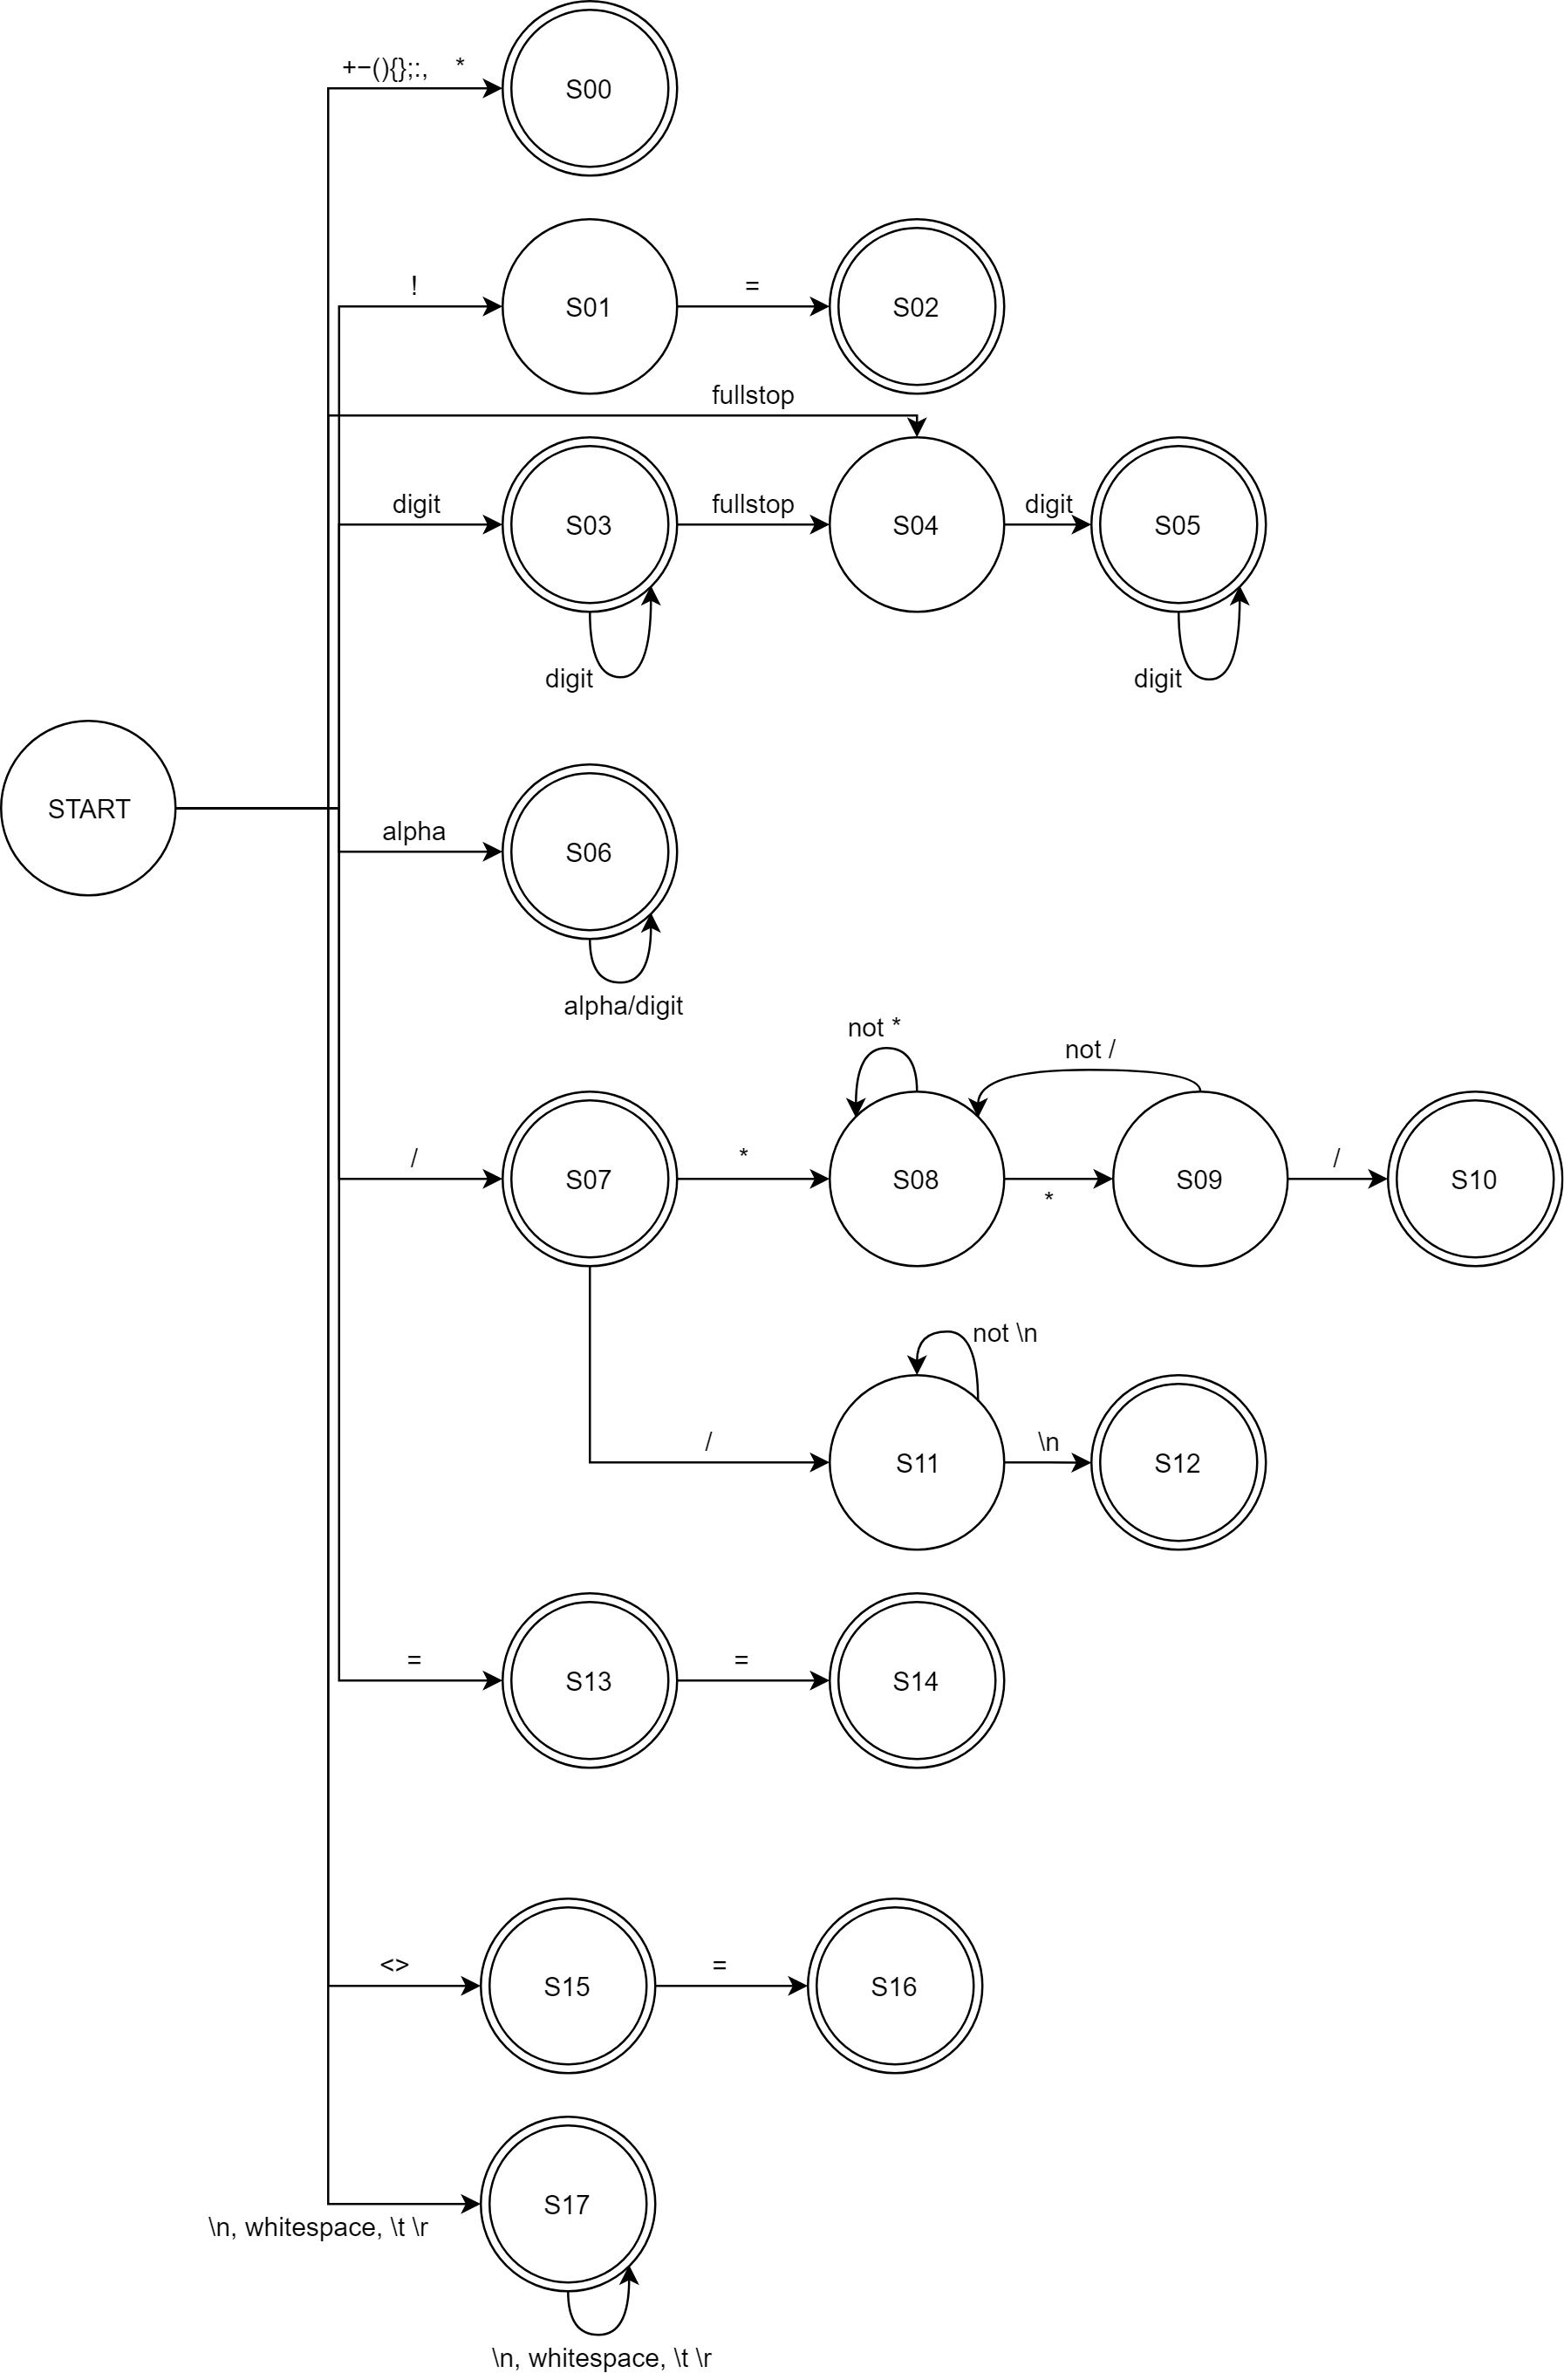
\includegraphics[width=\textwidth]{Images/Q1_StateTransitionDiagram.png}
	\caption{DFA for Lexer}
\end{figure}

As a table, it would look something like this:
\begin{lstlisting}[language=C]
asdasdas
\end{lstlisting}

\textbf{Note:} ST is the start state and SE is the error state

If the program goes to SE (the error state), then the lexeme is over. If the current state is not a final state, then an error is reported and Lexical Analysis stops. If if the program goes to SE and is in a final state, then the lexeme is kept and tokenized with a type.

The token class is the following (Found in the Token.h file):
\begin{lstlisting}[language=C++]
class Token{
	public:
		static enum TokenType{
			ID, BOOL, FLOAT, INT, // ID and constants
			ST, SE, GT, GE, EQQ, NE, AND, OR, NOT, // conditional operators
			EQ, PLUS, MINUS, TIMES, DIVISION, //arithmetic operators
			IF, ELSE, FOR, WHILE, FN, RETURN, TYPE_BOOL, TYPE_FLOAT, TYPE_INT, VAR, //keywords
			COLON, SEMI_COLON, COMMA, //punctuation
			OPEN_CURVED_BRACKET, CLOSED_CURVED_BRACKET, OPEN_CURLY_BRACKET, CLOSED_CURLY_BRACKET, //brackets punctuation
			COMMENT
		};
		TokenType type;
		string text = "";
		float number;
};
\end{lstlisting}

The final states result in some token. The following is a list of which states can result to which tokens (based on the lexeme).
\begin{enumerate}
	\item S0: PLUS, OPEN\textunderscore BRACKET, CLOSED\textunderscore BRACKET, OPEN\textunderscore BRACE, CLOSED\textunderscore BRACE, COLON, SEMI\textunderscore COLON, COMMA, TIMES
	\item S2: NE
	\item S3: INT
	\item S5: FLOAT
	\item S6: ID (or one of mykeywords[] below)
	\item S7: ID
	\item S8: DIVISION
	\item S12: COMMENT
	\item S15: COMMENT
	\item S16: EQ
	\item S17: EQQ
	\item S18: GT, ST
	\item S19: GE, SE
\end{enumerate}

The array of keywords in Token.cpp is as follows:
\begin{lstlisting} [language=C++]
// Used to check if a given string is a keyword (or identifier), and what type of keyword it is
struct Keyword{
	string text;
	Token::TokenType tok_type;
};

Keyword mykeywords[] = {
	{"and", Token::AND},
	{"or", Token::OR},
	{"not", Token::NOT},
	{"if", Token::IF},
	{"else", Token::ELSE},
	{"for", Token::FOR},
	{"while", Token::WHILE},
	{"fn", Token::FN},
	{"return", Token::RETURN},
	{"bool", Token::BOOL},
	{"float", Token::FLOAT},
	{"int", Token::INT},
	{"var", Token::VAR},
	{"true", Token::BOOL},
	{"false", Token::BOOL}
};
\end{lstlisting}